\maketitle

\section*{Data-provenance correction to versions 1--2}
An independent reader alerted the author that the 81,088-pair input used for
the observational analysis in versions 1--2 was named
\texttt{Newton\_dr3\_MSMS\_d200pc\_5.csv}.  A subsequent audit confirmed that
the redistributed reduction matches Chae's official virtual Newtonian v5
catalogue, rather than the real Gaia DR3 catalogue.  Consequently, all
observational results in the original Section 5 are withdrawn, including the
quoted $\gamma=1.05$, $\Delta\ln\mathcal L=129$, the associated
$\sim16\sigma$ statement, and the claimed deep-bin exclusion.  They cannot be
interpreted as measurements of the sky.  This revision uses the complete
81,880-pair real catalogue with corrected RUWE from Zenodo record 10986733,
separates the surviving synthetic result from the corrected observational
application, and reports failed validation controls rather than overriding
them.  Full forensic details are supplied with the reproducibility package.

\begin{abstract}
We study the sensitivity of wide-binary gravity estimators to residual
hierarchical triples and eccentricity modelling.  Known-truth catalogues are
constructed from Keplerian binaries and hierarchical triples, with Gaia-like
noise and the upstream velocity selection.  On Newtonian truth with a residual
triple fraction of 0.2--0.3, a full-median estimator recovers
$\gamma=G_{\rm eff}/G_{\rm N}=1.062$--$1.128$, whereas a tail-truncated
estimator gives 1.002--1.044 and a binary--triple mixture likelihood gives
0.98--1.00.  When $\gamma=1.4$ is injected above 2 kau, the latter two
estimators give 1.306--1.346 and 1.36--1.40.  This supports a methodological
claim: residual triple tails can create a positive bias in a full-median
estimator, while matched truncation or explicit mixture modelling reduces it.
The corrected real-data application uses Chae's 81,880-pair Gaia catalogue with
corrected RUWE.  In the 2--30 kau zone, the truncated estimator gives
$1.084\,[1.063,1.105]$ for empirical per-zone eccentricities but
$1.007\,[0.987,1.023]$ for a thermal distribution; the corresponding mixture
fits give 1.13 and 1.01.  Crucially, the empirical and superthermal branches
fail the pre-specified 2 per cent validation-zone control, while the thermal
branch passes.  Deep-bin estimates span 1.22--1.31 with broad 68 per cent
intervals.  The corrected Gaia DR3 outcome is therefore model-dependent and
non-conclusive under the pre-registered decision logic.  No high-significance
observational gravity verdict is claimed.
\end{abstract}

\section{Introduction}
Wide binaries probe internal accelerations near and below
$a_0\simeq1.2\times10^{-10}\,{\rm m\,s^{-2}}$.  Some MOND external-field
calculations predict $\gamma\simeq1.35$--1.40, corresponding to an approximately
18 per cent velocity increase, whereas Newtonian gravity predicts $\gamma=1$.
Analyses of Gaia DR3 have reached conflicting conclusions (e.g. Chae 2023,
2024; Banik et al. 2024; Pittordis et al. 2025).  Selection, unresolved
multiplicity, eccentricity distributions, and perspective corrections can all
be coupled to the inferred gravity parameter.

This paper has two distinct aims.  First, we perform an injection--recovery
comparison of estimator families on synthetic universes of known truth.
Second, we apply the same pipeline to a corrected real Gaia catalogue while
enforcing a validation-zone control.  These aims must remain separate: success
on a simulated Newtonian catalogue is a calibration result, not a measurement
of the gravitational field in nature.

\section{Catalogue provenance and audit}
The original scripts read an 81,088-row file derived from
\texttt{Newton\_dr3\_MSMS\_d200pc\_5.csv}.  Chae's public Zenodo records
identify the \texttt{Newton\_*} family as virtual catalogues whose astrometric
distances and proper motions are replaced by simulated Newtonian orbits and
hidden companions.  Source identifiers and several static columns remain tied
to the real catalogue, which made a superficial identifier match insufficient
to establish observational provenance.

Our audit joins the repository reduction to both the official v5 mock and the
real catalogue by the two Gaia source identifiers.  All 81,088 rows and all 19
analysis columns of the reduction agree with the v5 mock at relative tolerance
$10^{-9}$.  As an independent fingerprint, the median
$|d_1-d_M|$ is 0.000768 pc in the legacy file and 0.137569 pc in the real
catalogue; 94.19 per cent of legacy pairs, but only 8.42 per cent of real pairs,
lie within the projected orbital line-of-sight offset.  The relative proper
motions have correlation 0.626 with their real-catalogue counterparts.

For the corrected analysis we use the full
\texttt{gaia\_dr3\_MSMS\_d200pc\_ruwe.csv} table from Zenodo record 10986733:
81,880 rows and MD5 \texttt{1b6c5063163a4e6c07043d13aeb70f55}.  This release
also corrects the previously mismatched RUWE information.  The loader verifies
the URL, filename, digest, schema and row count, and refuses both
\texttt{Newton\_*} inputs and the 81,088-row fingerprint.

\section{Observable and corrected pipeline}
The dimensionless projected velocity is
\begin{equation}
 \vt=\frac{|\Delta v_\perp|}{\sqrt{G_{\rm N}M_{\rm tot}/s_{\rm 2D}}}.
\end{equation}
We use an angular perspective correction evaluated at the common mean distance.
Missing radial velocities are explicitly masked, and radial-velocity
uncertainty is propagated through the change of sky basis.  A trial $\gamma$
is applied to the model velocity before measurement noise, the upstream
El-Badry-type velocity cut, and the estimator cut.  In a hierarchical triple it
scales the low-acceleration outer orbit only; compact inner photocentre motion
remains Newtonian.

The fiducial selection requires distance below 200 pc,
$R_{\rm chance}<0.01$, RUWE below 1.4 for both components, and
$\sigma_{\vt}<0.10$.  It retains 38,472 pairs.  The validation zone
$0.2\le s_{\rm 2D}<2$ kau contains 28,221 pairs, the test zone
$2\le s_{\rm 2D}<30$ kau contains 7,900, and the deep bin
$0.03\le\gN/a_0<0.3$ contains 403.  A strict RUWE cut of 1.2 retains 31,264
pairs.  The perspective correction is small in the validation zone but not for
the widest systems: the 90th percentile of $|\Delta\vt|$ is 0.00172, 0.0286,
and 0.224 in the validation, test, and deep zones respectively.

We compare three eccentricity families: empirical per-zone values supplied in
the catalogue, thermal, and superthermal.  The primary truncated estimator E2
uses medians below $T=\sqrt{2}$ in data and zone-matched noisy templates.  The
secondary estimator E3 maximizes a Poisson likelihood over $(\gamma,\ftrip)$
for a binary plus hierarchical-triple mixture.  Intervals reported for E2 are
the central 68 per cent of 400 bootstrap resamples.  E3 intervals use the
profile-likelihood $\Delta\ln\mathcal L=0.5$ contour.  These are conditional
intervals within each specified model, not a complete systematic uncertainty.

\section{Synthetic injection--recovery}
The population engine follows the Keplerian binary and hierarchical-triple
construction described in Pittordis et al. (2025), including photocentre motion
and averaging over the Gaia DR3 time baseline.  It reproduces the principal
published validation statistics without tuning.  Synthetic catalogues use
noise resampled from the corrected real table.  Common random orbital
realisations are used across the gravity grid, and $\gamma$ is applied before
noise and selection.

We generate
$\gamma\in\{1.0,1.4\}$, three eccentricity prescriptions and
$\ftrip\in\{0,0.1,0.2,0.3\}$.  E1 is a validation-calibrated ratio of full
medians; E2 applies the matched $\vt<\sqrt2$ truncation; E3 fits binary and
triple histograms jointly.

\begin{figure*}
\centering
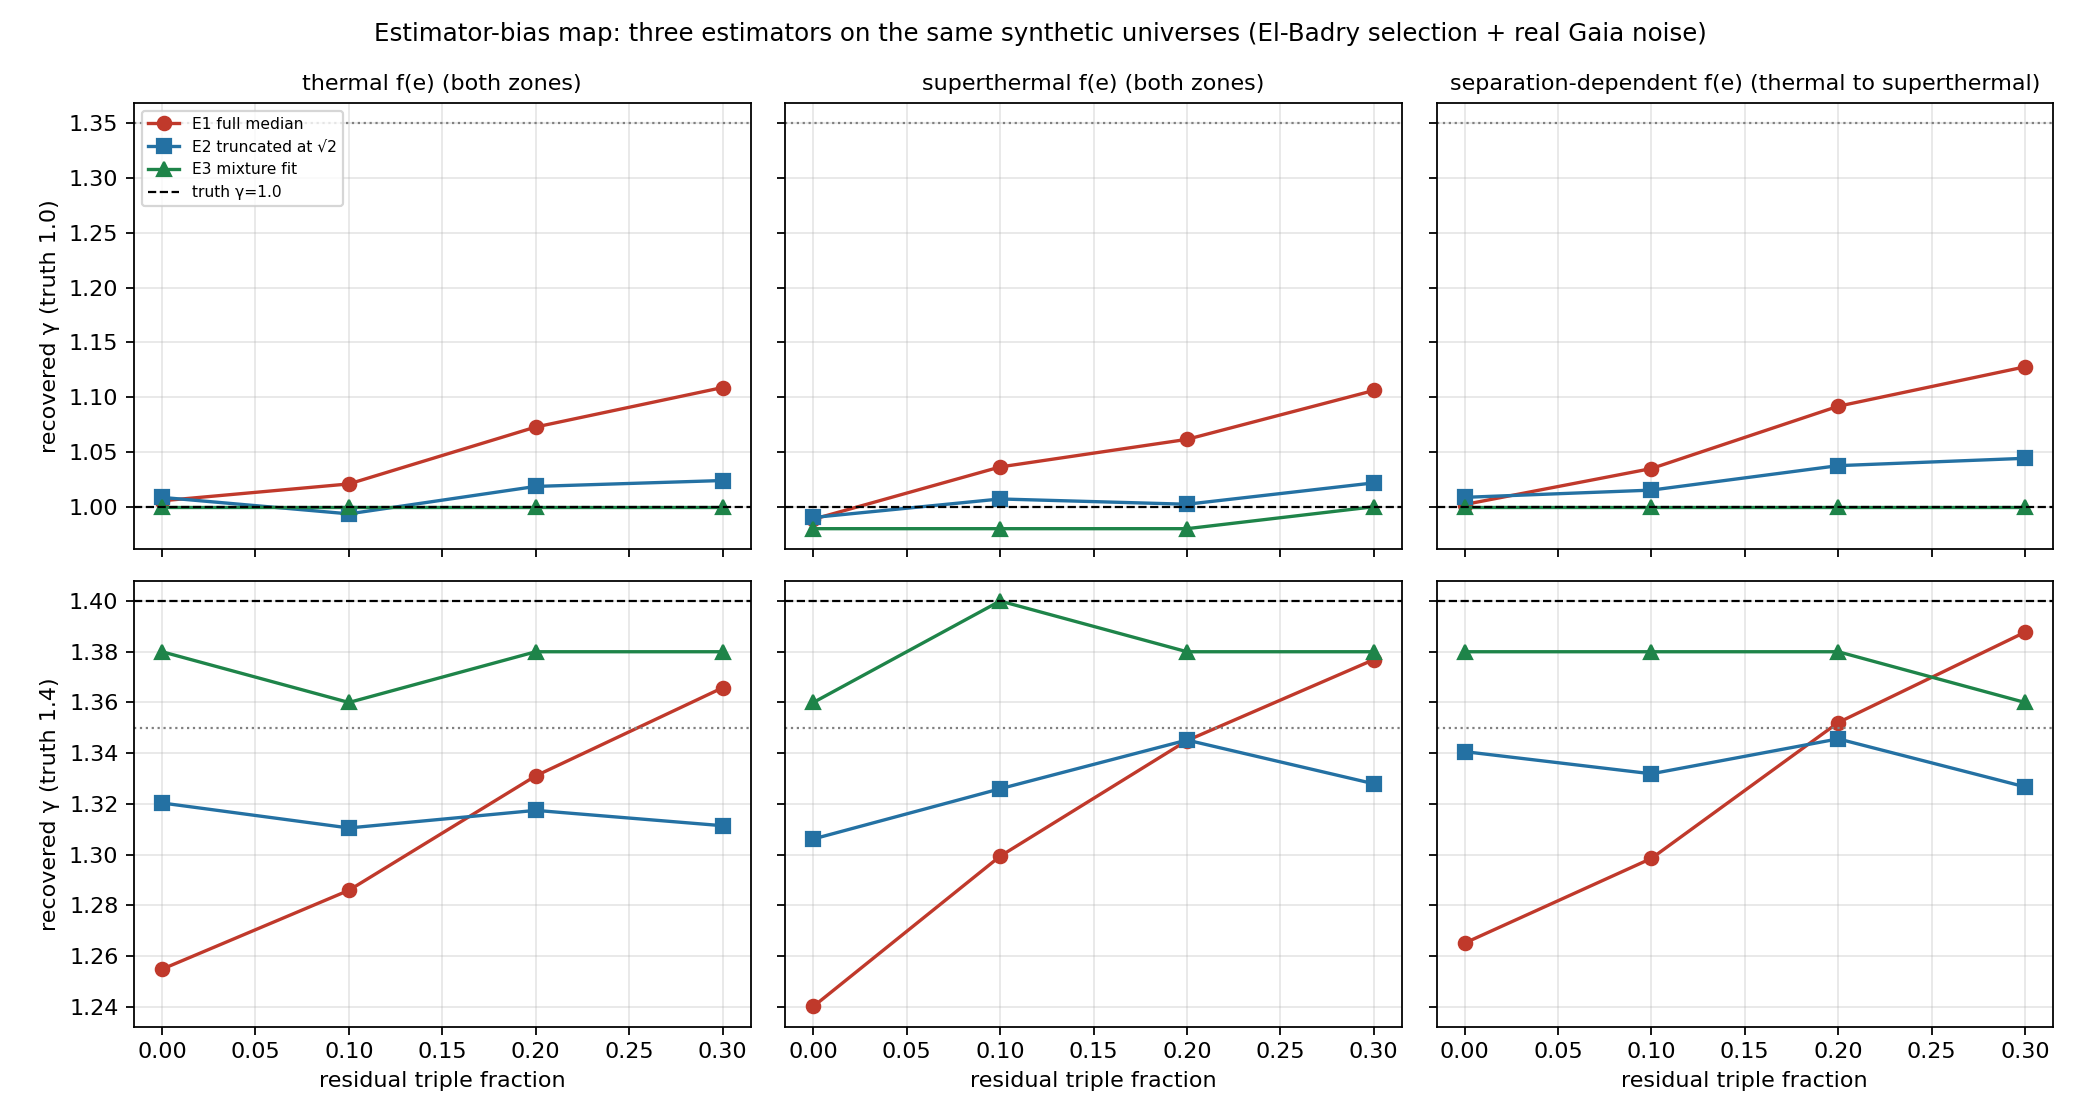
\includegraphics[width=\textwidth]{figures/figure_maitresse_G_corrected.png}
\caption{Corrected known-truth injection--recovery grid.  The rows show
Newtonian and $\gamma=1.4$ truth; columns show the eccentricity prescriptions.
The full-median estimator becomes positively biased as the triple fraction
increases.  The truncated and mixture estimators better separate the two
gravity regimes.}
\label{fig:synthetic}
\end{figure*}

For Newtonian truth at $\ftrip=0.2$--0.3, E1 gives 1.062--1.128, E2 gives
1.002--1.044, and E3 gives 0.98--1.00.  For injected $\gamma=1.4$, over all
triple fractions, E2 gives 1.306--1.346 and E3 gives 1.36--1.40; E1 gives
1.240--1.388.  Thus the synthetic experiment supports an estimator-bias
diagnosis, but its single-seed grid and simplified triple population do not by
themselves establish the astrophysical triple fraction or the gravity law.

\section{Corrected Gaia DR3 application}
The mandatory validation control compares the observed validation-zone median
to its Newtonian template and requires agreement within 2 per cent.  Table
\ref{tab:corrected} shows that only the thermal branch passes.  The empirical
branch used for the original primary analysis misses the control by 10.99 per
cent and must stop under the pre-registered logic.

\begin{table*}
\centering
\caption{Corrected real-catalogue results at $T=\sqrt2$.  Bracketed ranges are
68 per cent conditional intervals.  A failed validation branch is reported for
diagnosis, not used for a gravity verdict.}
\label{tab:corrected}
\small
\begin{tabular}{lcccc}
\hline
$f(e)$ model & validation offset & E2: 2--30 kau & E2: deep bin & E3: $\gamma$; $\ftrip$\\
\hline
empirical & $+10.99\%$ (fail) & $1.084\,[1.063,1.105]$ & $1.308\,[1.232,1.418]$ & $1.13\,[1.13,1.14]$; 0.14\\
thermal & $+1.77\%$ (pass) & $1.007\,[0.987,1.023]$ & $1.221\,[1.132,1.316]$ & $1.01\,[1.00,1.02]$; 0.16\\
superthermal & $+4.06\%$ (fail) & $1.007\,[0.988,1.022]$ & $1.222\,[1.146,1.314]$ & $1.04\,[1.02,1.05]$; 0.15\\
\hline
\end{tabular}
\end{table*}

The global E2 estimate changes little when the RUWE threshold is tightened:
the empirical, thermal and superthermal values become 1.067, 0.996 and 0.996.
Scanning $T=1.2$--1.8 gives 1.084--1.098 for the empirical family and
1.001--1.021 for thermal/superthermal families.  This threshold stability does
not remove the much larger eccentricity-model dependence or repair a failed
validation control.

\begin{figure*}
\centering
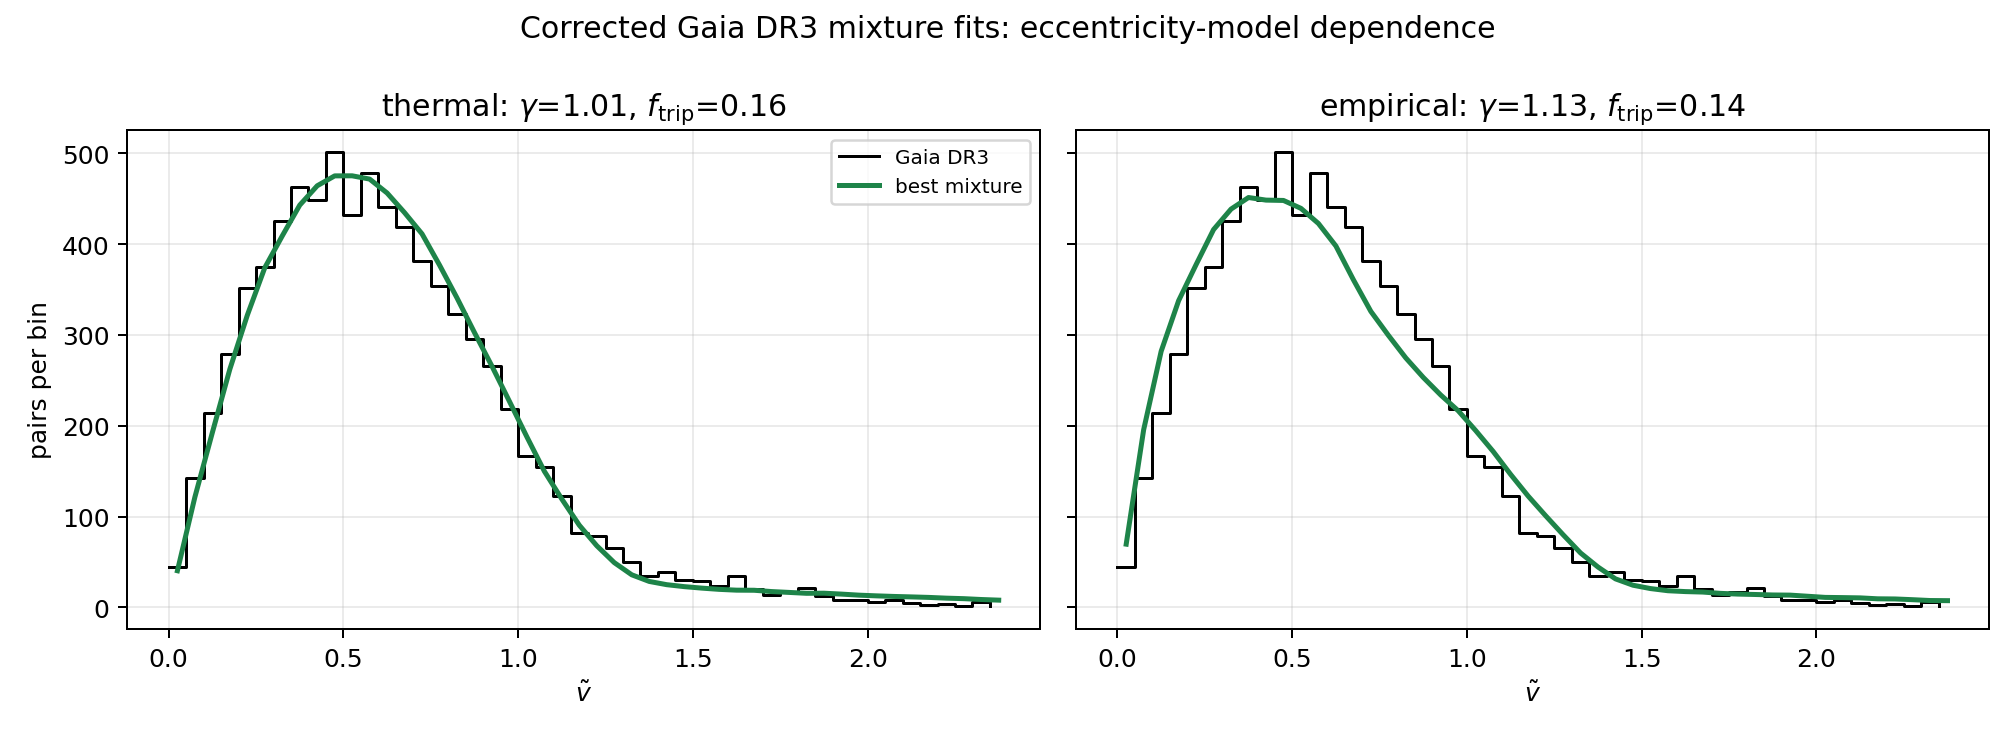
\includegraphics[width=0.96\textwidth]{figures/fig2_mixture_fit_corrected.png}
\caption{Corrected Gaia DR3 mixture fits for thermal (left) and empirical
(right) eccentricity prescriptions.  The difference between panels is a model
sensitivity, not an observational detection.}
\label{fig:mixture}
\end{figure*}

The E3 best fits similarly depend on the eccentricity prescription.  Although
the conditional likelihood strongly disfavors $\gamma=1.4$ in the thermal and
superthermal implementations, quoting this as a model-independent significance
would be inappropriate: the empirical branch shifts the best fit and fails the
validation control, and the likelihood does not marginalize over the full
eccentricity and triple-population uncertainty.

\begin{figure}[!htb]
\centering
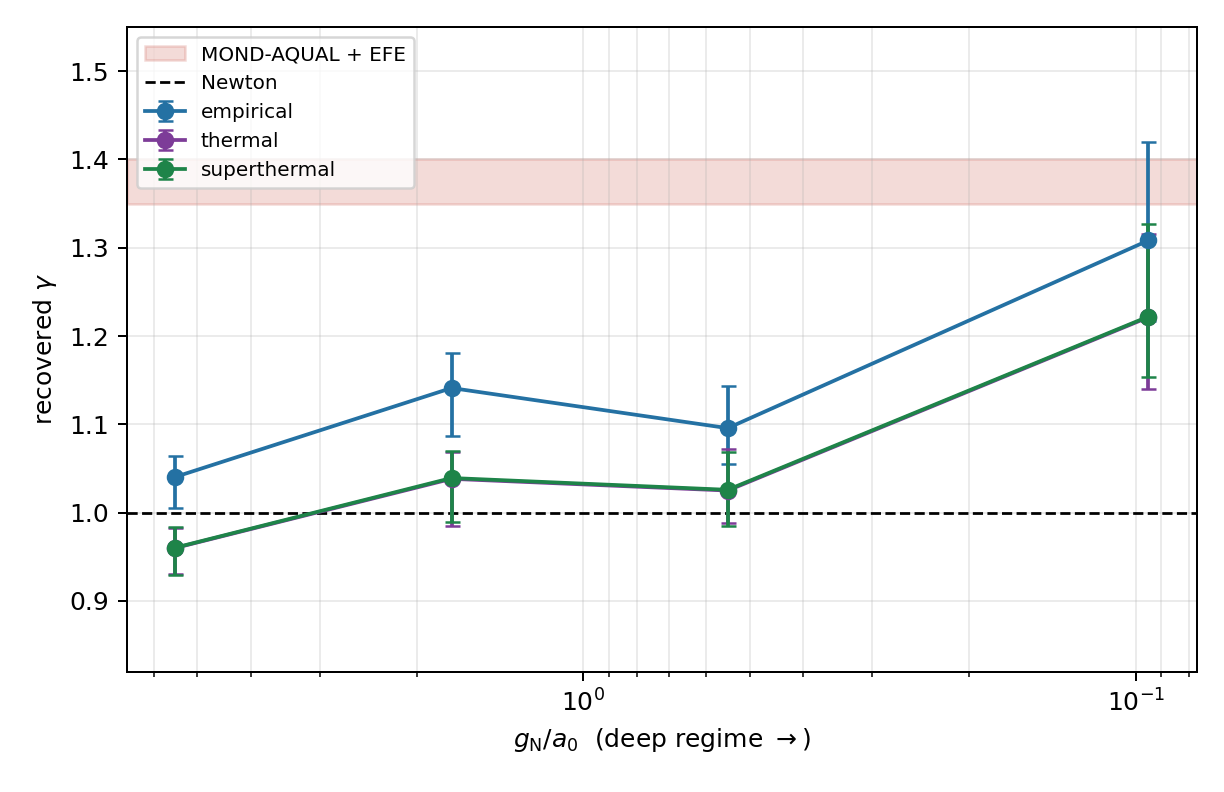
\includegraphics[width=\accelerationfigurewidth]{figures/fig3_gamma_vs_gN_corrected.png}
\caption{E2 estimates versus internal acceleration for the three eccentricity
families.  The divergence and broad deep-bin intervals motivate the
non-conclusive classification.}
\label{fig:acceleration}
\end{figure}

In the deep bin, the 68 per cent ranges are 1.232--1.418 (empirical),
1.132--1.316 (thermal) and 1.146--1.314 (superthermal).  Perspective effects are
large there, and the sample contains only 403 pairs.  These conditional results
do not justify the previous claim that the MOND-EFE range is excluded.  Taken
together, the failed controls and model spread place the corrected DR3
application in the pre-declared grey/non-conclusive category.

\section{Implications for the DR4 protocol}
The original pre-registration file is retained unchanged as a historical
record, but its DR3 calibration paragraph is invalid because it inherited the
mock-catalogue analysis.  A dated pre-DR4 amendment removes that calibration
standard, adds mandatory source-identity and checksum checks, records
the gravity-ordering correction for triples, and requires propagation of
radial-velocity uncertainty.  It does not use or anticipate a Gaia DR4 outcome.

The most important surviving rule is the STOP condition: a failed Newtonian
validation zone is a pipeline result that must be published, not tuned away.
The present exercise demonstrates why model families and validation outcomes
must be shown individually rather than compressed into a nominal statistical
significance.

\section{Conclusions}
Versions 1--2 confused a virtual Newtonian catalogue with observational Gaia
data.  Their Section 5 gravity measurement and significance claims are
withdrawn.  Reanalysis of the corrected real catalogue produces materially
model-dependent results; only the thermal eccentricity branch passes the
specified validation control, and the deep bin is not decisive.  This work
therefore makes no high-significance claim for either Newtonian or modified
gravity from Gaia DR3.

The narrower synthetic conclusion survives.  In known-truth experiments,
residual triple tails bias a full-median estimator upward, while matched
truncation and explicit mixture modelling reduce the bias and distinguish the
simulated Newtonian and $\gamma=1.4$ regimes.  Whether those models adequately
describe the sky remains a separate astrophysical question for better data and
pre-registered validation with Gaia DR4.

\section*{Data and code availability}
The corrected code, provenance audit, machine-readable outputs, legacy
quarantine, and DR4 amendment are available at
\url{https://github.com/HBoufourou/paperI-wide-binaries}.  Versions 1--2 are
archived at Zenodo DOI \url{https://doi.org/10.5281/zenodo.22114321}; they are
affected by the error described here.  The corrected release DOI will be added
after a new Zenodo version is minted.  The real Gaia-derived catalogue is
downloaded from Zenodo record 10986733 and checksum-verified by the pipeline.

\section*{Acknowledgements}
The author thanks the independent reader who identified the provenance issue
and supplied a reproducible audit.  Naming is deferred until consent for public
acknowledgement is obtained.  The author also thanks Andrei Tokovinin for
comments on an earlier version.  This work received no external funding.

\section*{Declaration on computational tools}
Large language models were used as computational and analytical assistants to
write, debug and audit scripts and text.  The provenance finding was
independently reproduced from public files and is recorded in executable code.
The author is responsible for the assumptions, interpretation, correction and
publication decisions.

\begin{thebibliography}{99}
\bibitem{BanikZhao2018} Banik I., Zhao H., 2018, MNRAS, 480, 2660
\bibitem{Banik2024} Banik I., Pittordis C., Sutherland W., et al., 2024, MNRAS, 527, 4573
\bibitem{Banik2026} Banik I., et al., 2026, arXiv:2602.24035
\bibitem{Chae2023} Chae K.-H., 2023, ApJ, 952, 128
\bibitem{Chae2024} Chae K.-H., 2024, ApJ, 960, 114
\bibitem{ElBadry2019} El-Badry K., 2019, MNRAS, 482, 5018
\bibitem{ElBadry2021} El-Badry K., Rix H.-W., Heintz T. M., 2021, MNRAS, 506, 2269
\bibitem{Hernandez2024} Hernandez X., et al., 2024, MNRAS, 533, 729
\bibitem{Hwang2022} Hwang H.-C., Ting Y.-S., Zakamska N. L., 2022, MNRAS, 512, 3383
\bibitem{Offner2023} Offner S. S. R., Moe M., Kratter K. M., et al., 2023, ASPC, 534, 275
\bibitem{Pittordis2018} Pittordis C., Sutherland W., 2018, MNRAS, 480, 1778
\bibitem{Pittordis2023} Pittordis C., Sutherland W., 2023, OJAp, 6, 4
\bibitem{PS25} Pittordis C., Sutherland W., Shepherd P., 2025, arXiv:2504.07569
\bibitem{Tokovinin2014} Tokovinin A., 2014, AJ, 147, 87
\end{thebibliography}
